\documentclass[10pt,UTF8]{ctexart}


\usepackage[margin=2cm,a4paper]{geometry}
%\usepackage[left=0.75in,top=0.6in,right=0.75in,bottom=1.0in,a4paper]{geometry}

\setmainfont{Caladea}
%% 也可以選用其它字庫:
% \setCJKmainfont[%
%   ItalicFont=AR PL KaitiM GB,
%   BoldFont=Noto Sans CJK SC,
% ]{Noto Serif CJK SC}
% \setCJKsansfont{Noto Sans CJK SC}
% \renewcommand{\kaishu}{\CJKfontspec{AR PL KaitiM GB}}

% 繁體中文
\setCJKmainfont[Path=fonts/ ]{NotoSansTC-Medium.otf}

\usepackage{minted}
\usepackage[breaklinks]{hyperref}

% Picture
% 導言區的此三行無變化
\usepackage{graphicx}
\usepackage{float} 
\usepackage{subfigure}
% 以下是新增的自定義格式更改
\usepackage[]{caption2} %新增調用的宏包
\renewcommand{\figurename}{Fig.} %重定義編號前綴詞
\renewcommand{\captionlabeldelim}{.~} %重定義分隔符
 %\roman 是羅馬數字編號,\alph是默認的字母編號,\arabic是阿拉伯數字編號,可按需替換下一行的相應位置
\renewcommand{\thesubfigure}{(\roman{subfigure})}%此外,還可設置圖編號顯示格式,加括號或者不加括號
\makeatletter \renewcommand{\@thesubfigure}{\thesubfigure \space}%子圖編號與名稱的間隔設置
\renewcommand{\p@subfigure}{} \makeatother

% Math
\usepackage {mathtools}
\usepackage{amssymb}

% Code
\usepackage{listings}
\usepackage{xcolor}
\lstset{
    % backgroundcolor=\color{red!50!green!50!blue!50},
    % 程式碼塊背景色為淺灰色
    rulesepcolor= \color{gray}, % 程式碼塊邊框顏色
    breaklines=true,  % 程式碼過長則換行
    numbers=left, % 行號在左側顯示
    numberstyle= \small,% 行號字型
    % eywordstyle= \color{red,% 關鍵字顏色
    commentstyle=\color{gray}, % 註釋顏色
    frame=shadowbox % 用方框框住程式碼塊
    }

\usepackage{hyperref}

\title{計算機視覺作業}
\author{干皓丞,2101212850, 信息工程學院}

\begin{document}
\maketitle


\section{作業目標與章節摘要}

在 GitHub 的 eriklindernoren/PyTorch-GAN 專案中選一個感興趣的 GAN 程式,下載並運行,寫出閱讀總結,並對應程式碼標註出公式以及網路所對應的程式碼。(詳細說明,不超過兩頁)

\section{作業說明與實際狀況}

作業可以從 GitHub 下的 kancheng/kan-cs-report-in-2021 專案找到,作業程式碼目錄為 kan-cs-report-in-2021/CV/gans/code。在過程中實際執行過的 GAN 程式碼有 cgan.py、cluster\_gan.py、dcgan.py、gan.py、infogan.py、lsgan.py 、sgan.py,而當中 cluster\_gan.py 因為實驗環境配置問題並沒有順利執行,而其他的方法皆穩定執行,所以在此選擇 infogan.py 執行並進行說明,其 infogan.py 則來自 2016 年的發表 'InfoGAN: Interpretable Representation Learning by Information Maximizing Generative Adversarial Nets',實驗設備為 MacBook Pro (Retina, 15-inch, Mid 2014) 和 Acer Aspire R7。

InfoGAN 是一個基於生成對抗網絡所修改的方法,該方法是無監督來進行解決問題,同時最大化了潛在變量的小子集與觀察之間的互信息。其原文解釋為 (also maximizes the mutual information between a small subset of the latent variables and the observation),而互信息(mutual information)字面解釋為共有的資訊。

\begin{figure}[H]
\centering 
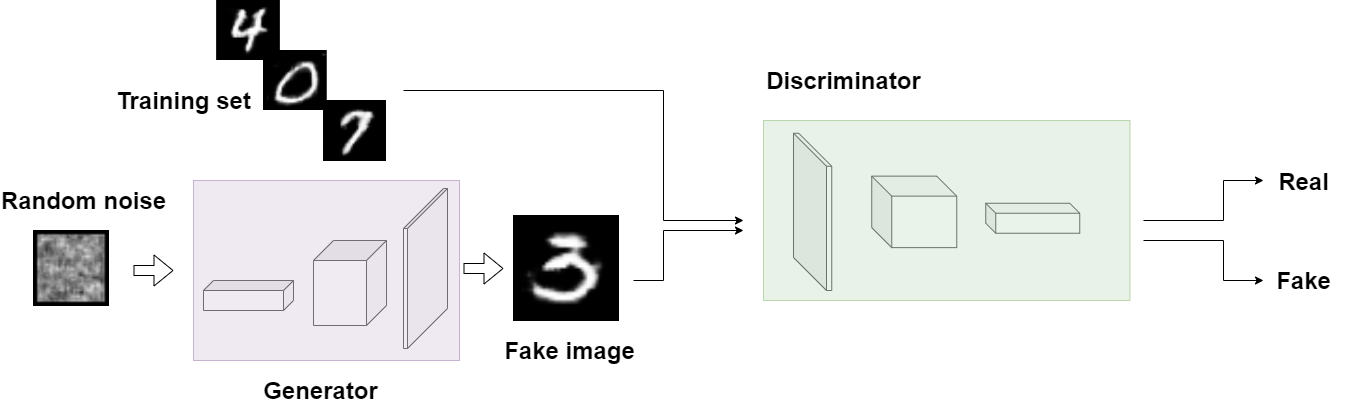
\includegraphics[width=0.80\textwidth]{su1.png} 
\caption{說明示意}
\label{Test}
\end{figure}
\begin{figure}[H]
\centering 
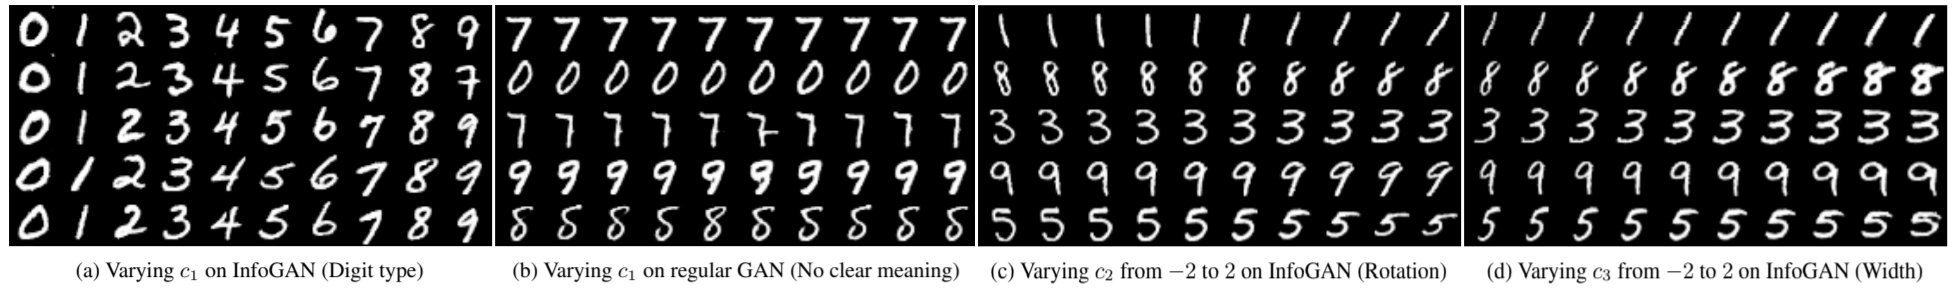
\includegraphics[width=0.80\textwidth]{su2.png} 
\caption{研究呈現}
\label{Test}
\end{figure}
數學意義說明則可以在第四節、第五節與附錄中找到,研究中所提出的的 Value 函數如下 :

$$\min \limits_{G}\max \limits_{D}{V_I(D,\ G)=V(D,G)-\lambda L_I(G,Q)}$$

從研究中可以知道,若相互對 c 進行約束,c 對生成資料若越 Interpretable Representation, 則 c 和 G 的相關性越高,若無相關性,則相互之間的 I 趨於零。 Value 函數的對抗中,期望互信息I(c; G(z,c))越大越好。

訓練中通過調整參數,可以觀察到過程中產生的資料,從程式碼執行的結果看,確定能區分書數字的傾斜度、粗細、數字,而從研究中的 7.2 Disentangled Representation 可以看到 Figure 2: Manipulating latent codes on MNIST 的呈現, (a) 中,c1 中的每一屬性表示一個數字; (c) 中的 c2 屬性的範圍,則表示傾斜度、小-左傾、大-右傾;(d) 中,c3 屬性表示粗細。而專案程式碼一開始的順序大略分為 9 大部分。

	\begin{lstlisting}[language={python}]
Step 1. 準備階段,包含套件匯入、建立 3 個輸出目錄、Python 指令介面、叫 GPU 。
Step 2. 函數定義與設計,包含 weights\_init\_normal 初始定義,to\_categorical 分類,定義 Generator(nn.Module): [Generator],定義 Discriminator(nn.Module): [Discriminator]。
Step 3. 定義損失函數 - adversarial\_loss(MSELoss())、categorical\_loss(CrossEntropyLoss())、continuous\_loss (MSELoss())。
Step 4. Loss weights 調整參數 - lambda\_cat = 1 ;lambda\_con = 0.1
Step 5. 初始 (Initialize) 準備 Generator and Discriminator ( 詳見 7. and 8.)、GPU CUDA 判斷、資料載入,包含當中 Generator 和 Discriminator 的 weights
Step 6. 資料載入
Step 7. 設定 Optimizers 的 generator 和 discriminator,當中還有一個 itertools 做迭代,使用 Adam。
Step 8. 設定 Generator 輸出與存圖
Step 9. 做訓練並分為四大部分 (1) Train Generator(2) Train Discriminator(3) Information Loss(4) Log Progress
	\end{lstlisting}
	對應上面程式碼,下圖為 InfoGAN 運作原理,輸入資料(Z)分為兩部分,假設有 40 項,前 20 為 Z-C,後 20 項為 Z-Z',若為手寫任務, Z-C 為筆畫格式, Z-Z' 為 隨機,Classifier 是抓 Generator 輸出 X 下,原本輸入的 Z-C 是什麼。同時 Discriminator 則是查 Generator 輸出 X 是否是 True image,同時 Classifier 和 Generator 之間的關係像類似 encoder 和 decoder 之間的 Auto-encoder 關係,但與傳統 Auto-encoder 差異在於,傳統是圖轉轉成編碼後,再轉成圖,InfoGAN 則是輸入編碼轉圖後,再轉成編碼。在此過程中 Discriminator 必須是要存在。同時 Discriminator 也與 Classifier 共享參數。
\begin{figure}[H]
\centering 
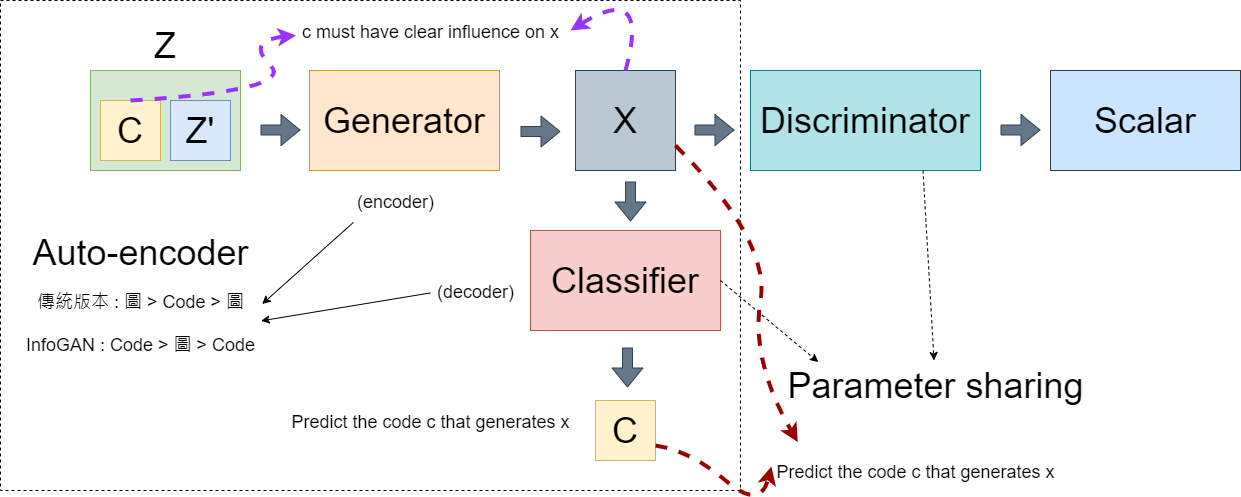
\includegraphics[width=0.80\textwidth]{su3.png} 
\caption{InfoGAN}
\label{Test}
\end{figure}
%\begin{enumerate}
%\item Y
%\item A
%\end{enumerate}

% \newpage

\clearpage

\end{document}